\chapter{Análise dos Resultados da Fase 1}

\section{Avaliação da confiabilidade}

Primeiramente, foi executado uma avaliação de confiabilidade para o formulário proposto. O método de avaliação utilizado foi o alfa de Cronbach. Para encontar o $\alpha$ foi utilizada a fórmula definida no capítulo de Metodologias.

O cálculo foi aplicado somente as questões de escala de classificação em que a escala de avaliação varia entre 1 e 5.

O cálculo do $\alpha$ de Cronbach gerou um valor exato de 0.753268, e este valor é classificado como "Alto", segundo os valores referenciados no capítulo de Metodologias. 

\section{Interpretação dos dados}

O mapa de calor a seguir, gerado pelo ChatGPT, representa as correlações entre diferentes formatos de feedback com base nas preferências dos alunos. Cada célula representa a correlação entre dois formatos de feedback, com valores variando de -1 a 1. Um valor de correlação próximo de 1 indica uma forte correlação positiva, significando que quando a preferência por um formato aumenta, a preferência pelo outro também tende a aumentar. Um valor próximo de -1 indicaria uma forte correlação negativa, o que não é observado neste conjunto de dados. Valores próximos de 0 indicam pouca ou nenhuma correlação.

\begin{figure}[H]
\centering
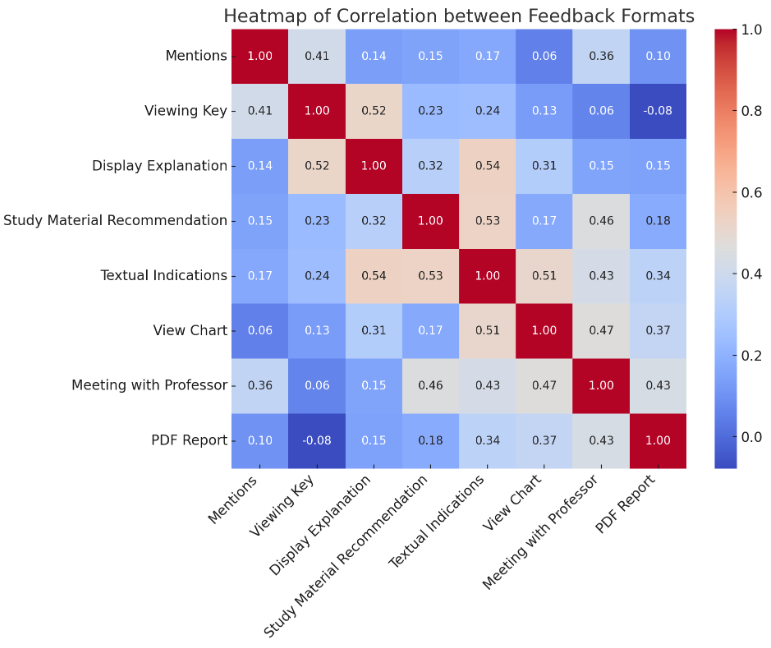
\includegraphics{figuras/heatmapfeedback.png}
\caption{Mapa de calor das correlações entre os formatos de feedback}
\end{figure}

A partir dos dados quantitativos, obtidos através do formulário, é possivel extrair diversas informações qualitativas relevantes, tais como: 

1. Explicação do gabarito de cada questão: Esse aspecto parece ser bastante valorizado, com muitos 5's, indicando que os respondentes veem grande importância em entender o porquê de suas respostas estarem certas ou erradas.

2. Indicação do material de estudo: Este item parece ter uma importância moderada a alta, com uma variação nas respostas, mas com muitos participantes ainda atribuindo a nota máxima.

3. Correlações mais fortes entre certos formatos, como explicação de gabarito e indicação de material de estudo, podem sugerir que os alunos veem esses métodos como complementares e eficazes em conjunto.

4. As respostas às questões visualizar gabarito de cada questão, explicação do gabarito, e indicação de material de estudo indicam uma preferência dos alunos por feedbacks que fornecem detalhes específicos e orientações claras. Isso sugere que os alunos valorizam feedbacks que não apenas apontam os erros, mas também orientam sobre como corrigi-los e melhorar.

5. As preferências mais baixas para temas com baixa taxa de acerto e gráfico de desempenho) podem indicar que, embora a visualização de dados seja útil, ela deve ser complementada com feedbacks mais explicativos e detalhados para ser eficaz.

6. As correlações observadas entre diferentes formatos de feedback sugerem que um sistema de IA para feedback formativo deve ser capaz de identificar padrões nos erros dos alunos e fornecer explicações detalhadas, juntamente com recursos e orientações para melhoria.

7. A IA poderia ser programada para reconhecer áreas problemáticas comuns entre os alunos e sugerir recursos específicos ou estratégias de estudo.

8. Visualizar Gabarito e Explicação do Gabarito: A alta preferência por esses formatos indica que os alunos valorizam não só saber as respostas corretas, mas também entender o raciocínio por trás delas. Isso sugere a importância de um sistema de IA que não se limite a apontar erros, mas forneça explicações claras e métodos para corrigi-los.

9. As correlações entre diferentes formatos de feedback apontam para a preferência dos alunos por um sistema holístico que integre múltiplos tipos de feedback. Por exemplo, a combinação de visualização de desempenho com explicações detalhadas pode ser particularmente eficaz.

10. Variação Mínima: As variações nas preferências de feedback com base no gênero são mínimas para a maioria dos formatos, indicando que ambos os gêneros têm preferências similares por esses tipos de feedback.

\begin{figure}[H]
\centering
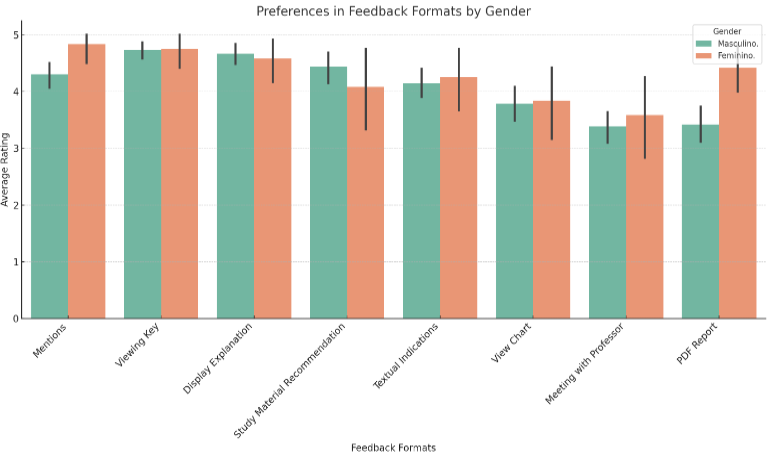
\includegraphics{figuras/gender_graph.png}
\caption{Gráfico representando a relação entre gênero e a avaliação do formato de feedback.}
\end{figure}

11. Algumas correlações entre diferentes formatos de feedback foram moderadamente altas, indicando que os alunos que preferem um tipo de feedback também tendem a preferir outros tipos similares. Por exemplo, a correlação entre Explicação do Gabarito e Indicação de Material de Estudo foi particularmente notável.

12. Foi observada correlações moderadas entre a presença de transtornos neurobiológicos e a preferência por certos tipos de feedback, como "Visualizar Gabarito" e "Reunião com o Professor". Essas correlações sugerem que alunos com transtornos neurobiológicos podem ter preferências específicas por feedbacks mais detalhados e interativos.

O gráfico a seguir, gerado pela ferramenta ChatGPT, mostra as correlações entre a presença de transtornos neurobiológicos nos respondentes e suas preferências por diferentes formatos de feedback:

\begin{figure}[!h]
\centering
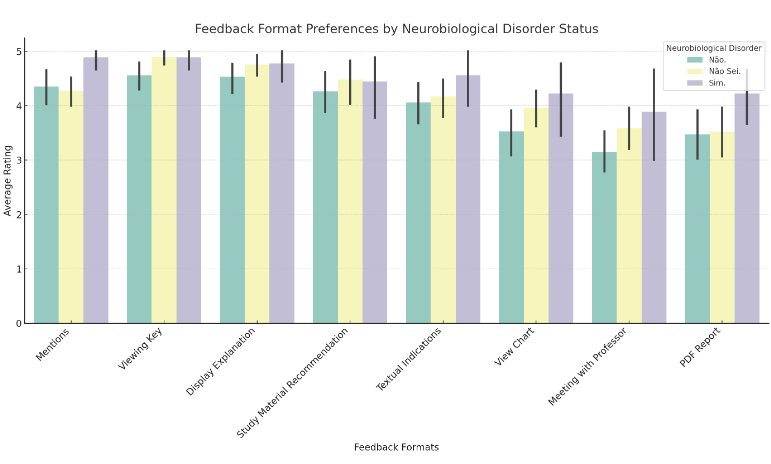
\includegraphics{figuras/neurological_graphic.png}
\caption{Correlações entre a presença de transtornos neurobiológicos nos respondentes e suas preferências por diferentes formatos de feedback}
\end{figure}

\begin{table}[H]
\centering
\begin{tabular}{|c|p{6cm}|p{8cm}|}
\hline
\textbf{Nº} & \textbf{Aspecto Analisado} & \textbf{Observações e Conclusões} \\
\hline
1 & Explicação do Gabarito de Cada Questão & Alta valorização com muitos 5's, indicando a importância de entender as respostas certas ou erradas. \\
\hline
2 & Indicação do Material de Estudo & Importância moderada a alta, com variação nas respostas. \\
\hline
3 & Correlação entre Explicação de Gabarito e Material de Estudo & Sugere que os alunos veem esses métodos como complementares. \\
\hline
4 & Preferência por Feedbacks Detalhados e Orientações Claras & Alunos valorizam feedbacks que orientam sobre como corrigir erros e melhorar. \\
\hline
5 & Preferências mais Baixas para Temas com Baixa Taxa de Acerto & Indica que feedbacks devem ser complementados com detalhes explicativos. \\
\hline
6 & Correlações entre Formatos de Feedback & Sistema de IA deve identificar padrões nos erros e fornecer explicações detalhadas e recursos para melhoria. \\
\hline
7 & IA para Reconhecimento de Áreas Problemáticas & Sugerir recursos específicos ou estratégias de estudo. \\
\hline
8 & Visualizar Gabarito e Explicação do Gabarito & Alta preferência indica a valorização do entendimento do raciocínio por trás das respostas. \\
\hline
9 & Correlações entre Diferentes Formatos de Feedback & Preferência por um sistema holístico que integre múltiplos tipos de feedback. \\
\hline
10 & Variação Mínima com Base no Gênero & Preferências similares entre os gêneros para a maioria dos formatos de feedback. \\
\hline
11 & Correlações entre Diferentes Tipos de Feedback & Alunos que preferem um tipo de feedback tendem a preferir outros similares. \\
\hline
12 & Correlações e Transtornos Neurobiológicos & Alunos com transtornos neurobiológicos podem preferir feedbacks mais detalhados e interativos. \\
\hline
\end{tabular}
\caption{Resumo das Análises dos Dados Quantitativos do Formulário}
\end{table}


\section{Discussão}

A partir dos dados apresentados, os três formatos de feedback com maior dominância de importância foram: "Visualizar o gabarito de cada questão", "Exibir a explicação correspondente ao gabarito de cada questão" e "Indicação do material de estudo necessário para revisões do conteúdo". Estes três formatos corroboram com a ideia de feedback formativo, que, segundo Shute \cite{shute2008focus}, é definido como a informação comunicada ao aluno que pretende modificar seu pensamento ou comportamento com o propósito de melhorar o aprendizado, ou seja, consiste em toda informação que permite ao aluno identificar o que falta fazer e como fazer para alcançar o esperado.

Também é importante considerar as limitações deste estudo. Primeiramente, a amostra foi limitada a alunos de duas disciplinas específicas, o que pode restringir a generalização dos resultados para outros contextos educacionais ou disciplinas. Além disso, o estudo focou principalmente em correlações entre preferências de feedback e certos fatores demográficos, como gênero e a presença de transtornos neurobiológicos, mas não explorou outras variáveis importantes que podem influenciar as preferências de feedback, como o contexto cultural, o histórico educacional prévio ou o estilo de aprendizagem individual.